\documentclass[conference,a4paper]{IEEEtran}
\usepackage[T1]{fontenc}
\usepackage{amsmath,amssymb,graphicx,booktabs,cite,url}
\usepackage[hidelinks]{hyperref}
\graphicspath{{figures/}}
\title{Domain-Separated Evaluation of Character CNN--BiLSTM Phishing Detection: A Reproducibility Study}
\author{\IEEEauthorblockN{D Sunidhi, P Manvitha, G Likith}
\IEEEauthorblockA{Department of Computer Science and Information Technology\\KLH Bachupally}}
\begin{document}\maketitle
\begin{abstract}
Phishing-model revisions can improve a demonstration while invalidating earlier evaluation claims. We audit an independently developed URL detector as it evolves from a character CNN--LightGBM ensemble to a character CNN, bidirectional LSTM and additive-attention network. Executable partition reconstruction identifies registered-domain overlap and two cleaned training-input matches in an external snapshot. We repair the split by assigning complete registered-domain groups, sharing cleaning-based exclusion keys, reserving previously evaluated domains, and freezing the protocol before a single retraining run. The retained data comprise 25,961 training, 6,113 validation and 31,795 test rows, with zero pairwise public- and private-suffix domain intersections. The corrected candidate obtains 92.876\% accuracy, 90.696\% recall and 98.289\% ROC-AUC on its disjoint test partition at threshold 0.5. Comparisons on common external and synthetic-stress inputs expose both benefits and regressions rather than transferring historical headline metrics. The frozen validation promotion gate failed; production remains the separately identified v3.3 model. Independent inert HTML/email analysis and reviewed feedback provide prototype extensions, not additional validated classifier probabilities. The contribution is an auditable implementation and evaluation correction, not a novel recurrent algorithm or prospective temporal benchmark.
\end{abstract}
\begin{IEEEkeywords}phishing detection, bidirectional LSTM, character CNN, domain separation, reproducibility, evaluation leakage\end{IEEEkeywords}

\section{Introduction}
URL phishing detectors must classify strings that change over time and distinguish malicious structures from legitimate authentication paths. A model can obtain excellent results on one curated split yet flag familiar development or account URLs. This discrepancy may reflect source bias, input preprocessing, architecture, the decision threshold, or evaluation leakage. It cannot be resolved scientifically by assuming that a larger dataset or a more complex neural layer must help.

Dubey \emph{et al.}~\cite{phishx} propose a character CNN and engineered-feature LightGBM ensemble. Their article reports 99.819\% accuracy and 100\% precision on its own test set. Our first independent 20,000-URL reproduction obtained 99.525\% accuracy. Neither figure describes the presently served classifier. Subsequent production work changed the data, encoding, ensemble weights and ultimately the architecture. This paper studies that evolution through preserved code, checkpoints, prediction records and an explicit repair experiment.

The research question is: \emph{what performance and integrity conclusions survive an audit of the latest hybrid sequence detector and a whole-domain repartitioning?} We separate software correctness, numerical reproducibility, dataset independence and deployment selection. A passing API test is not evidence of unseen-domain generalization. A maintainer's production choice is not proof that a recorded research gate passed.

Our contributions are threefold. First, we trace the exact deployed CNN--BiLSTM--attention network and its relationship to historical ensemble scores. Second, we identify a fixed-row reservation defect, repair it with whole-group assignment and frozen assertions, and train one versioned candidate without changing architecture or threshold. Third, we report same-input clean, external and synthetic-stress comparisons with explicit membership limitations, alongside independent context and reviewed-adaptation infrastructure. These are reproducibility and systems contributions rather than inventions of convolution, recurrence, attention or grouped splitting.

\section{Related Work}
URL-based detection predates modern deep learning. Garera \emph{et al.}~\cite{garera} examine phishing detection and measurement, while Blum \emph{et al.}~\cite{blum} study lexical URL learning with online adaptation. URLNet~\cite{urlnet} learns character- and word-level representations. Yang \emph{et al.}~\cite{yang} investigate multidimensional phishing features. Our original baseline follows PhishX~\cite{phishx} and uses LightGBM~\cite{lightgbm}; the latest verdict does not continue that probability fusion.

Character convolution~\cite{charconv} motivates local symbol-pattern extraction. LSTM~\cite{lstm} provides gated recurrence, and bidirectional recurrence~\cite{brnn} combines both sequence directions. Learned alignment~\cite{attention} motivates weighted aggregation, although our scalar additive pooling is not the full translation attention architecture. These established methods explain the latest network's capabilities, not a claim of algorithmic novelty or an isolated causal improvement from one layer.

SpacePhish~\cite{spacephish} and gray-box phishing work~\cite{graybox} distinguish realistic attack capabilities from arbitrary perturbations. Our deterministic string mutations are a narrower stress model and are not checked against live pages. PhishIntention~\cite{phishintention} uses webpage appearance and behavior; our pasted-text context tools are not equivalent learned vision or interaction systems. Security-ML evaluation guidance~\cite{arp} and TESSERACT~\cite{tesseract} motivate independent partitions and temporal caution. Human review of feedback is motivated by poisoning concerns~\cite{poisoning}, but we do not claim experimentally demonstrated poisoning resistance.

\section{Proposed Methodology}
\subsection{Versioned Data and Domain Integrity}
The first reproduction sampled 10,000 legitimate and 10,000 phishing URLs from frozen PhishX snapshots whose provenance names Tranco and PhishTank~\cite{tranco,phishtank,phishxcode}. Its final 14,002/2,000/3,998 split was registered-domain-disjoint. Later V2 data contain 40,000 balanced rows. v3.3 adds 24,000 source-derived records: 12,000 phishing URLs, 9,000 legitimate paths and 3,000 lower-ranked Tranco roots. These are source labels rather than new labels established by visiting destinations.

The v3.3 trainer claimed grouped evaluation but assigned some hard negatives and previous test URLs individually before grouping the remaining rows. Another URL from an already reserved hostname could therefore be assigned elsewhere. Reconstruction yields hostname intersections of 11, 40 and 6 and private-suffix registered-domain intersections of 385, 400 and 187 for train--validation, train--test and validation--test. Public-suffix intersections are 439, 458 and 229. Zero exact URL-key overlap did not imply domain separation. Two fresh2 URLs also became identical to training inputs after scrape-artifact cleaning, exposing inconsistent exclusion semantics.

The repaired v3.4 pipeline uses an offline bundled public-suffix list and assigns whole public registered-domain groups. This deliberately keeps tenants of private hosting suffixes together; it is stricter than tenant-level grouping. IP hosts are grouped by their normalized address. Cleaning repairs known scraping escapes, filters malformed records and applies a shared conservative identity key. Source files remain unchanged. The new identity policy removes 50 duplicates after 81 invalid rows, retaining 63,869 records; the former trainer removed 46 duplicates.

Reservations apply to complete groups with deterministic priority test $>$ validation $>$ training. Domains present in earlier held-out, adversarial and frozen external evaluation sources are kept out of candidate training. StratifiedGroupKFold with seed 42 assigns the remaining domains. This resolves 85 reservation conflicts without moving a test domain into training to improve balance. Consequently, the final proportions differ from the nominal 70/15/15 allocation of unreserved groups. Table~\ref{tab:split} reports actual counts. Hashes of data, assignments and implementation are committed before training; pairwise intersections are asserted for keys, hostnames and both suffix interpretations.

\begin{table}[t]\centering\small
\caption{Frozen v3.4 Partitions; All Pairwise Domain Intersections Are Zero}\label{tab:split}
\begin{tabular}{lrrr}\toprule
Split & Legitimate & Phishing & Total\\\midrule
Train & 13,612 & 12,349 & 25,961\\
Validation & 3,220 & 2,893 & 6,113\\
Test & 15,168 & 16,627 & 31,795\\\bottomrule
\end{tabular}\end{table}

\subsection{Feature Engineering and Historical Ensemble}
The historical baseline computes 36 string-only features: composition and lengths, URL structure, hostname/path entropy, suspicious-TLD indicators, six length buckets and nine keyword flags. Examples include digit-to-letter ratio, dots, path segments, percent encoding and login/verify terms. These are learned inputs, not a whitelist, ownership verification or DNS reputation service. The initial CNN uses 49 explicit symbols plus padding/unknown indices, length 200, lowercasing and rightmost truncation, embedding 16, three 128-filter convolutions and a 64-unit dense head.

The reference mixture is $p=0.6p_C+0.4p_L$. Validation selected 95/5 for the first reproduction, whereas production V2 later used separately trained models at 35/65. In current production the old CNN and calibrated LightGBM still produce reference scores, but their mixture does not determine the URL verdict. These distinctions prevent historical model names and metrics from being silently reassigned to a new artifact.

\begin{figure*}[t]\centering
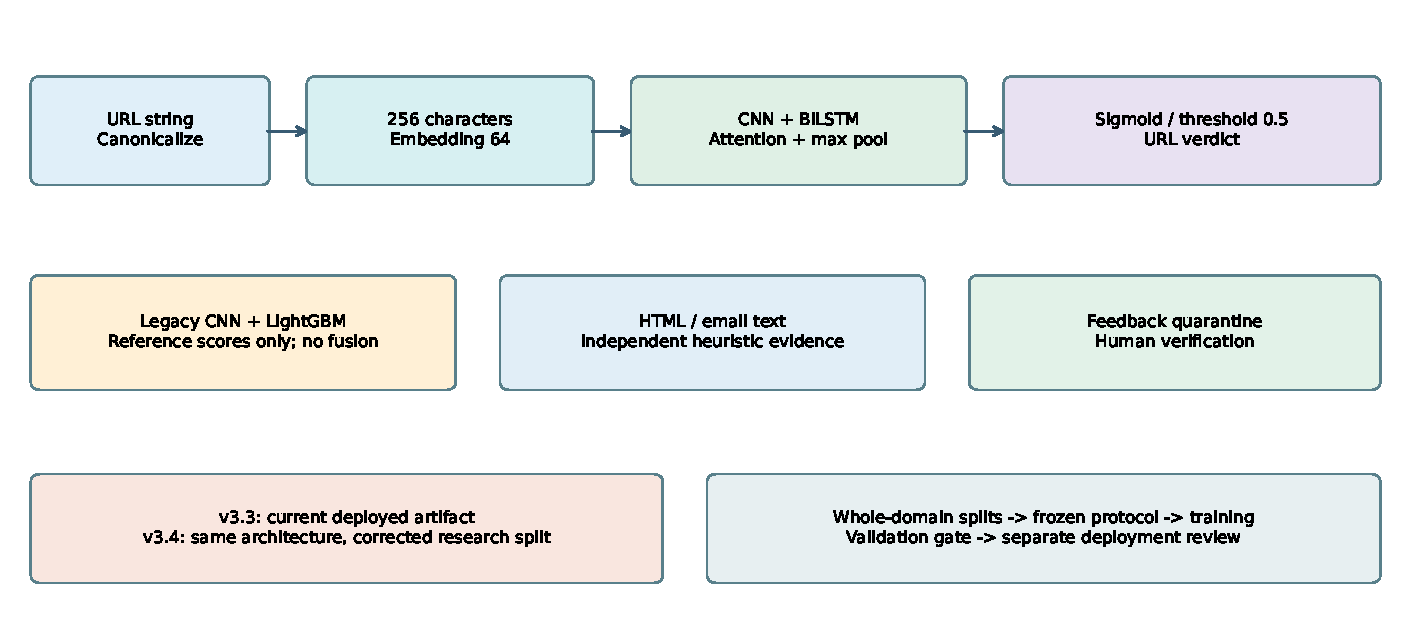
\includegraphics[width=\textwidth]{system_architecture.pdf}
\caption{Current neural decision path, reference-only legacy ensemble, and independent context/adaptation tools. v3.4 changes the evaluation/training partition, not the v3.3 layer structure. Deployment remains separately versioned.}\label{fig:system}
\end{figure*}

\subsection{Latest Sequence Architecture}
The encoder canonicalizes a URL as text, keeps its first 256 characters, and right-pads with zero. It uses 95 printable ASCII characters, padding 0 and unknown 96: 97 indices. Unlike the original encoder, path/query case is preserved. Root slash normalization, scheme/host case and missing-scheme handling are shared with serving; meaningful path slashes, queries and fragments remain intact. No submitted URL is fetched.

An embedding maps indices to 64 dimensions. Parallel Conv1D kernels 3, 5 and 7 each output 128 channels with batch normalization and ReLU. Concatenation yields 384 channels; stride-two max pooling leaves 128 time steps. A two-layer LSTM with hidden dimension 128 per direction has \texttt{bidirectional=True}. Dropout is 0.2 after convolution/pooling and between recurrent layers. Its per-step representation $h_t$ has 256 components. Additive pooling uses
\begin{equation}
e_t=w^\top\tanh(Wh_t+b),\quad
\alpha_t=\frac{\exp e_t}{\sum_j\exp e_j},\quad
c=\sum_t\alpha_t h_t.
\end{equation}
The score projection is 256--64--1. Concatenating $c$ with temporal max pooling produces 512 components. The head is 512--128--32--1, with LayerNorm, ReLU and dropout 0.3/0.15. A sigmoid and fixed 0.5 threshold produce the verdict. The network contains 1,138,434 parameters. It is additive attention pooling, not multi-head transformer attention; padding is not explicitly masked, and the sigmoid output has no separate fitted probability calibrator.

Bidirectionality can combine context on both sides of a pooled URL feature before classification. This is a plausible representational advantage over early global pooling, not evidence that it alone improved performance. v3.4 retains the architecture and optimizer settings to focus the repair on partition integrity, but changed training exposure still prevents an architecture-only causal comparison.

\subsection{Robustness, Context and Adaptation}
The preserved robustness framework supplies eight deterministic mutation families: path-token insertion, separator duplication, path-character percent encoding, subdomain addition, keyword splitting, punctuation insertion, query addition and path extension. The historical stress set contains 1,995 mutated phishing strings and 2,003 unchanged benign strings. Labels are inherited; destination validity and semantic equivalence are not proven. v3.4 is evaluated on this set but does not undergo new adversarial fine-tuning during the repair.

Standalone HTML and email endpoints parse only submitted text. HTML counts forms, passwords, scripts, iframes, redirects and credential-related terms. Email extracts implemented urgency, credential/call-to-action language and URL strings. Neither is a calibrated content classifier; neither changes the neural probability. Feedback is quarantined for human verification before an explicit offline learning workflow. A registry and PSI feature-drift monitor support governance, not an observed longitudinal learning benefit.

\section{Experimental Setup}
The protocol was frozen in local research commit \texttt{5543066} before the earlier candidate run. This output refresh performs no training. Seed 42, CPU execution with four Torch threads, batch size 128, AdamW learning rate $10^{-3}$, weight decay $10^{-4}$, BCEWithLogitsLoss and gradient clipping 5.0 match the existing recipe. The ceiling is seven epochs, early-stop patience three; ReduceLROnPlateau monitors validation AUC with factor 0.5 and patience one. Eligible training hard negatives retain the existing eightfold repetition rule; whole-domain reservations take priority. Checkpoint selection uses validation ROC-AUC only, retaining epoch 7. Validation loss is now saved alongside training loss and AUC.

The exported ONNX candidate is checked against its PyTorch checkpoint, and artifact hashes are preserved. Internal test probabilities are reused from the post-selection run rather than repeatedly selecting against that set. Comparisons score frozen V2, v3.3 and v3.4 artifacts at threshold 0.5. ROC-AUC and average precision accompany threshold metrics; precision--recall area here means average precision, not trapezoidal interpolation. No hyperparameter, threshold or ensemble-weight search uses these test outcomes.

The fresh2 snapshot has 11,273 rows; two exceed the serving limit of 2,048 normalized characters. The common API-compatible cohort therefore has 11,271 rows. These exclusions are explicit, not model-dependent error removal. Its domains are excluded from v3.4 training, but the snapshot has already influenced project development. It is not a newly collected blind temporal holdout. The earlier models have different training exposure to the corrected test and validation partitions; their comparison is diagnostic rather than an unbiased matched-training ablation.

The frozen candidate gate requires no reduction in corrected-validation ROC-AUC or phishing recall relative to v3.3, and at most a one-percentage-point benign-FPR increase. The gate failed. The branch does not automatically promote any artifact, even if a gate passes. Historical v3.3 was deployed by an explicit maintainer override after its own recall-gain gate failed; this is disclosed instead of rewritten as successful validation.

\section{Results and Discussion}
\subsection{Corrected Test Evaluation}
\begin{table}[t]\centering\small
\caption{Corrected Test (31,795 Rows); Percentages. Baselines Have Different Training Exposure.}\label{tab:test}
\setlength{\tabcolsep}{3pt}\begin{tabular}{lrrrrrr}\toprule
Model & Acc. & Prec. & Rec. & F1 & FP & FN\\\midrule
V2 ensemble & 56.172 & 54.500 & 98.045 & 70.057 & 13610 & 325\\
BiLSTM v3.3 & 97.500 & 98.262 & 96.933 & 97.593 & 285 & 510\\
Disjoint v3.4 & 92.876 & 95.455 & 90.696 & 93.015 & 718 & 1547\\
\bottomrule\end{tabular}\end{table}
The domain-separated candidate achieves 92.876\% accuracy, 95.455\% precision, 90.696\% recall, 93.015\% F1, 98.289\% ROC-AUC and 98.419\% average precision. It produces 718 false positives and 1547 false negatives. Table~\ref{tab:test} also reports older artifacts on identical test inputs, but their prior training exposure prevents interpreting their scores as equally independent estimates. Integrity and predictive performance must be reported separately: a valid split does not guarantee a larger score.

The original reproduction's 99.525\% accuracy and historical robust candidate's 99.625\% accuracy refer to 3,998 different test records and older architectures. The original paper's 99.819\% likewise comes from its own 19,873-record test. None is an appropriate numerical substitute for the repaired experiment. Direct superiority claims across these datasets would confound source composition, input representation, training size and sampling.

\subsection{External False-Positive Trade-offs}
\begin{table}[t]\centering\small
\caption{Previously Inspected Fresh2 Snapshot (11,271 Common API-Compatible Rows)}\label{tab:fresh}
\setlength{\tabcolsep}{3pt}\begin{tabular}{lrrrrrr}\toprule
Model & Acc. & Prec. & Rec. & F1 & FP & FN\\\midrule
V2 ensemble & 76.542 & 72.723 & 92.553 & 81.448 & 2177 & 467\\
BiLSTM v3.3 & 91.740 & 93.713 & 91.277 & 92.479 & 384 & 547\\
Disjoint v3.4 & 90.578 & 94.468 & 88.232 & 91.243 & 324 & 738\\
\bottomrule\end{tabular}\end{table}
Before repair, the replayed v3.3 reduced fresh2 false positives from 2,177 for V2 to 384, while false negatives rose from 467 to 547. Thus, higher accuracy did not mean higher phishing recall. The corrected v3.4 obtains 90.578\% accuracy and 88.232\% recall on the same API-compatible snapshot. Figure~\ref{fig:comparison} displays all three models without hiding the recall trade-off. Candidate training shares neither cleaned URL keys nor registered domains with this cohort, but prior inspection remains a study-level limitation.

\begin{figure}[t]\centering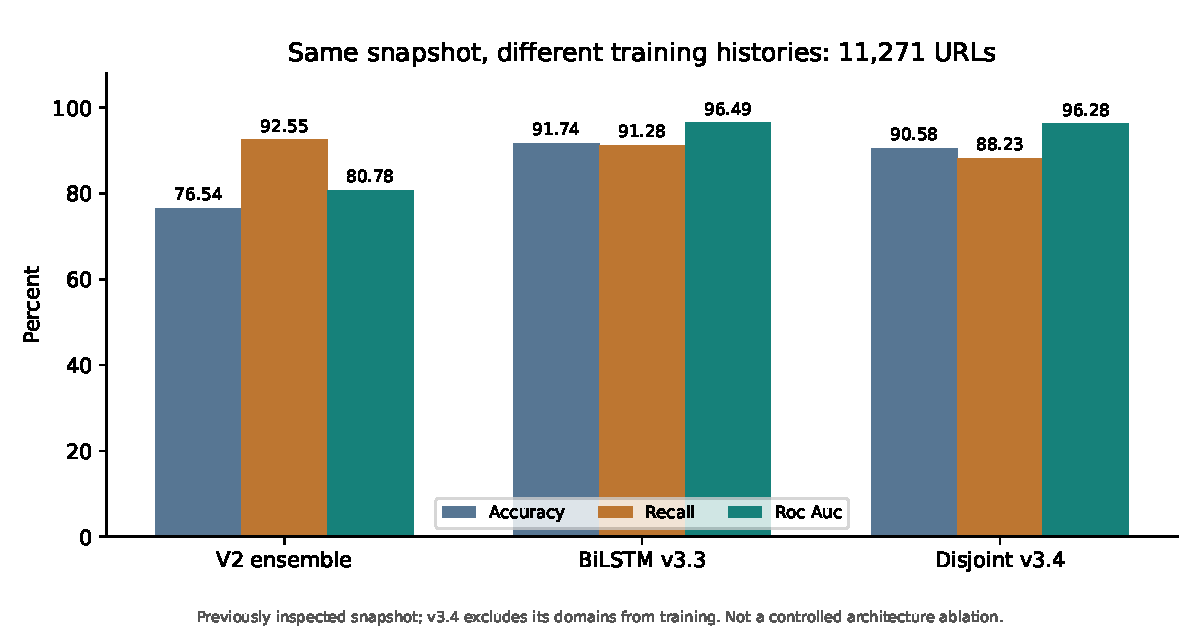
\includegraphics[width=\columnwidth]{model_comparison.pdf}
\caption{Common-input snapshot comparison. Training histories differ, and the snapshot was previously inspected.}\label{fig:comparison}\end{figure}

Saved and replayed classification counts match for the audited pre-repair models. Ranking metrics show small discrepancies: V2 ROC-AUC is 0.807826407 in batched replay versus 0.807972891 saved, with smaller differences in v3.2/v3.3. The cause is not established. We retain both records rather than silently replacing one or claiming bit-identical reproduction; the new figures use their associated replay scores.

\subsection{Synthetic Stress Evaluation}
\begin{table}[t]\centering\small
\caption{Historical Synthetic Stress Set (3,998 Rows)}\label{tab:adv}
\setlength{\tabcolsep}{3pt}\begin{tabular}{lrrrrrr}\toprule
Model & Acc. & Prec. & Rec. & F1 & FP & FN\\\midrule
V2 ensemble & 99.225 & 98.904 & 99.549 & 99.226 & 22 & 9\\
BiLSTM v3.3 & 96.273 & 98.426 & 94.035 & 96.180 & 30 & 119\\
Disjoint v3.4 & 95.373 & 99.346 & 91.328 & 95.168 & 12 & 173\\
\bottomrule\end{tabular}\end{table}
On the older 3,998-string stress set, V2 has 9 phishing misses and v3.3 has 119. The repaired candidate has 173 misses with 91.328\% recall. This comparison does not transfer the earlier robustness experiment's 37-to-17 improvement to a later architecture. The historical improvement remains valid only for its own saved baseline/candidate pair and synthetic generator. No result proves resistance to adaptive attackers, composed mutations or working live phishing pages.

\begin{figure}[t]\centering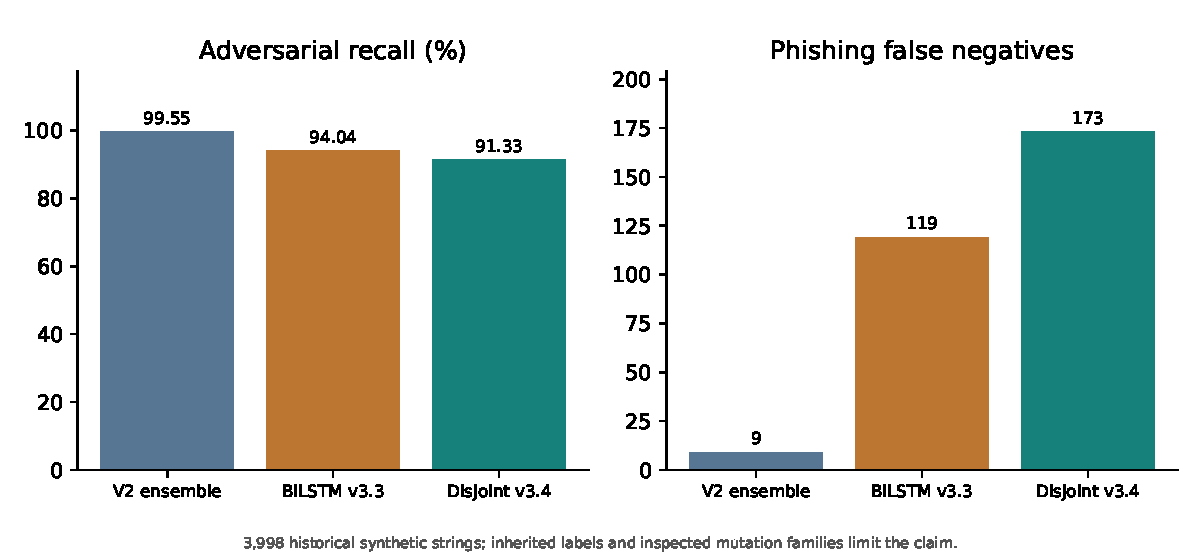
\includegraphics[width=\columnwidth]{adversarial_robustness.pdf}
\caption{Historical mutation-set replay. Counts and recall are shown together; v3.4 is not adversarially fine-tuned in this repair.}\label{fig:stress}\end{figure}

\subsection{Operational Interpretation}
The public service reports version \texttt{charcnn-bilstm-attention-v3.3}. Local/public health, prediction, standalone HTML/email, combined context and model-information routes were exercised. Google, GitHub and OpenAI root/slash pairs agree, and the synthetic suspicious string is submitted only to the detector API, never visited. Valid feedback was tested in an isolated local store; production validation was checked without inserting fabricated labels. The production-source suite passes 91 tests; the separate local research branch previously passed 107 including split regressions. Neither count is an accuracy certificate. Candidate binaries and training code remain local; this documentation release publishes the saved evidence, not a deployable v3.4 package.

The repaired pipeline prevents the specific pinned-row leakage defect and catches future group intersections before training. The corrected dataset retains fewer training examples because preserving known evaluation domains has priority. A fair future architecture study should retrain all baselines under the same partitions, with matched budgets and multiple seeds. This repair does not spend additional runs trying to win back a preferred headline score.

\section{Limitations}
The study uses inherited labels, historical source snapshots and balanced-source construction, not deployment prevalence. Even zero registered-domain overlap does not exclude shared campaigns, copied pages or semantic near-duplicates across domains. Public-suffix grouping is conservative and can hold out entire hosting providers, changing class and source composition. The large reserved test partition is intentional but not a random sample of future traffic.

The new experiment uses one seed and lacks a temporal holdout, recurrent ablations and confidence intervals. Earlier models have unequal exposure to the corrected partitions, so model-to-model differences are descriptive. Previously inspected snapshots cannot be made prospectively unseen by moving their domains out of a new training set. Synthetic labels are not independently verified, and mutation families are known from prior development.

Attention is not a causal explanation; displayed engineered features describe the URL but do not attribute the BiLSTM verdict. Unmasked padding, first-256 truncation and uncalibrated neural scores may affect behavior. HTML/email heuristics lack a labelled content evaluation, PSI thresholds lack longitudinal calibration, and reviewed feedback is not a proven poisoning defense. These limitations define useful future experiments rather than invalidating the narrow, reproducible observations reported here.

\section{Conclusion}
Auditing the latest phishing detector changed the research conclusion more substantially than changing its name from CNN to BiLSTM. We identified whole-domain leakage, inconsistent cleaned-input exclusions and a failed promotion criterion, then froze and executed a corrective training protocol. The v3.4 test result is 92.876\% accuracy and 90.696\% recall with zero pairwise registered-domain overlap; external and stress-set trade-offs are reported alongside it. Production remains v3.3, and historical ensemble results stay historical. The defensible contribution is a traceable model-and-evaluation pipeline with safe independent context tools, not a claim of universal detection or automatic improvement from architectural complexity.
\section*{Acknowledgment}
The authors acknowledge project guide Dr. K Venkateshwara Rao, KLH Bachupally.
\bibliographystyle{IEEEtran}\bibliography{references}
\end{document}
